%%%%%%%%%%%%%%%%%%%%%%%%%%%%%%%%%%%%%%%%%
% Beamer Presentation ; ML-Based Sensor Fusion for Indoor Localization
% Based on PLAN.md content, using THEME template style
%%%%%%%%%%%%%%%%%%%%%%%%%%%%%%%%%%%%%%%%%

\documentclass[
	11pt,
	aspectratio=169,
]{beamer}

\graphicspath{{img/}{THEME/Content/PPT_Pics/}{./}}

\usepackage{booktabs}
\usepackage{amsmath}
\usepackage{amssymb}
\usepackage{palatino}
\usepackage[default]{opensans}
\usepackage{tikz}
\usepackage{array}
\usepackage{multirow}
\usetikzlibrary{shapes.geometric, arrows.meta, positioning, calc, fit, backgrounds, decorations.markings}

%----------------------------------------------------------------------------------------
%	SELECT LAYOUT THEME
%----------------------------------------------------------------------------------------

\usetheme{Madrid}
\usecolortheme{whale}
\useinnertheme{circles}

\setbeamertemplate{navigation symbols}{}
\setbeamertemplate{caption}[numbered]

%----------------------------------------------------------------------------------------
%	ADD LOGO TO HEADER (matching theme)
%----------------------------------------------------------------------------------------

\addtobeamertemplate{frametitle}{}{%
  \begin{tikzpicture}[remember picture,overlay]
    \node[anchor=north east, inner sep=0pt, yshift=0.1cm, xshift=-0.3cm]
      at (current page.north east) {
\includegraphics[height=1.1cm]{logo.png}};
  \end{tikzpicture}%
}

%----------------------------------------------------------------------------------------
%	PRESENTATION INFORMATION
%----------------------------------------------------------------------------------------

\title[ML Sensor Fusion]{Asynchronous Sensor Fusion for ISAC Nodes Integrating Wi-Fi Sensing and mmWave Radar}
\subtitle{Edge-Deployed Neural Fusion on ESP32-S3 ISAC Nodes}

\author[VIT Chennai]{Avinash Nair (22BEC1435) \\ Anek Sreedhar (22BEC1376) \\ Akash Dasangam (22BEC1386) \\ \medskip \small Guide: Dr.\ Anith Nelleri}

\institute[]{Dept.\ of Electronics and Communication Engineering \\ \smallskip VIT Chennai}

\date[Mar 2026]{Review-3 \\ \today}

%----------------------------------------------------------------------------------------
%	TIKZ STYLES
%----------------------------------------------------------------------------------------

\tikzset{
  sysblock/.style={
    rectangle, rounded corners=3pt, draw=structure.fg!80, fill=structure.fg!8,
    minimum width=2.2cm, minimum height=0.9cm,
    text width=2cm, align=center, font=\scriptsize\bfseries
  },
  dataflow/.style={
    -Stealth, thick, draw=structure.fg!70
  },
  coreblock/.style={
    rectangle, rounded corners=2pt, draw=#1!80, fill=#1!8,
    minimum width=4.8cm, minimum height=3.2cm,
    text width=4.6cm, align=left, font=\tiny
  },
  coreblock/.default=blue,
  pipeblock/.style={
    rectangle, rounded corners=3pt, draw=structure.fg!80, fill=#1!12,
    minimum width=1.8cm, minimum height=0.7cm,
    text width=1.6cm, align=center, font=\tiny\bfseries
  },
  pipeblock/.default=blue,
  annot/.style={font=\tiny, text=gray!70!black},
}

%----------------------------------------------------------------------------------------

\begin{document}

%========================================================================================
%	SLIDE 1 ; TITLE
%========================================================================================

\begin{frame}[plain]
	\titlepage
\end{frame}

%========================================================================================
%	SLIDE 2 ; THE PROBLEM
%========================================================================================

\section{Problem \& Motivation}

\begin{frame}
	\frametitle{Why Sensor Fusion for Indoor Spaces?}
	\framesubtitle{GPS Fails Indoors ; Radar \& Wi-Fi Have Opposite Weaknesses}

	\begin{columns}[c]
		\begin{column}{0.50\textwidth}
			\scriptsize
			\textbf{The Gap:}
			\begin{itemize}
				\item GPS fails indoors ; warehouses, factories, hospitals have \alert{zero} satellite coverage
				\item 6G ISAC nodes combine communication + sensing on one device
				\item No single sensor works reliably alone
			\end{itemize}

			\medskip
			\textbf{Bottom line:} Radar is precise but blind behind walls. Wi-Fi sees through walls but is noisy. \alert{Fusing them} gives the best of both.
		\end{column}

		\begin{column}{0.47\textwidth}
			\centering
			\scriptsize
			\begin{tabular}{>{\raggedright}p{1.2cm} >{\centering}p{1.8cm} >{\centering\arraybackslash}p{1.8cm}}
				\toprule
				& \textbf{Radar} \newline (24\,GHz FMCW) & \textbf{Wi-Fi FTM} \newline (802.11mc) \\
				\midrule
				Precision & $\pm$0.15\,m & $\pm$1.5\,m \\
				Angle & Yes ($\pm$60$^{\circ}$) & No \\
				Through walls & \alert{No} & \alert{Yes} \\
				Update rate & 10--15\,Hz & $\sim$1--2\,Hz \\
				Identity & No & Yes \\
				\bottomrule
			\end{tabular}
		\end{column}
	\end{columns}
\end{frame}

%========================================================================================
%	SLIDE 3 ; OBJECTIVES
%========================================================================================

\begin{frame}
	\frametitle{Project Objectives}

	\begin{enumerate}
		\item Design a \textbf{hardware node} that performs radar + Wi-Fi sensing simultaneously
		\item Develop an \textbf{ML model} that learns to dynamically trust the better sensor
		\item Deploy the trained model directly on the \textbf{ESP32-S3} microcontroller (\alert{edge inference} ; no cloud)
		\item Validate that fused accuracy \textbf{beats either sensor alone} under occlusion
	\end{enumerate}

	\bigskip

	\begin{columns}[c]
		\begin{column}{0.45\textwidth}
			\begin{block}{Scope}
				Static indoor localization (fixed-position targets with micro-motion)
			\end{block}
		\end{column}
		\begin{column}{0.45\textwidth}
			\begin{exampleblock}{Coordinate System}
				Polar $(r, \theta)$ ; harmonizes radar's 2D output with Wi-Fi's range-only output
			\end{exampleblock}
		\end{column}
	\end{columns}
\end{frame}

%========================================================================================
%	SLIDE 4 ; HARDWARE ARCHITECTURE
%========================================================================================

\section{System Design}

\begin{frame}
	\frametitle{System Hardware}
	\framesubtitle{All OTS Components}

	\begin{columns}[c]
		\begin{column}{0.42\textwidth}
			\scriptsize
			\begin{block}{Sensing Node}
				\begin{itemize}
					\item \textbf{ESP32-S3} ; Dual-core LX7 @ 240\,MHz
					\item \textbf{HLK-LD2450} ; 24\,GHz FMCW radar, UART @ 256k baud, 10--15\,Hz
					\item Roles: FTM initiator + radar parser + \alert{ML inference engine}
				\end{itemize}
			\end{block}

			\begin{exampleblock}{Active Tag}
				\begin{itemize}
					\item \textbf{ESP32} ; FTM responder + ESP-NOW heartbeat
					\item Trihedral corner reflector ; boosts RCS, zero compute cost
				\end{itemize}
			\end{exampleblock}
		\end{column}

		\begin{column}{0.55\textwidth}
			\centering
			% TikZ Hardware Connection Diagram ; vertical layout
			\begin{tikzpicture}[scale=0.9, transform shape]
				\node[sysblock, fill=blue!12] (radar) {HLK-LD2450\\24\,GHz Radar};
				\node[sysblock, fill=green!12, below=1.0cm of radar] (esp) {ESP32-S3\\Sensor Node};
				\node[sysblock, fill=orange!12, below=1.0cm of esp] (tag) {ESP32\\Active Tag};

				\draw[dataflow] (radar) -- node[right, font=\tiny] {UART 256k} node[left, font=\tiny, text=gray] {GPIO16/17} (esp);
				\draw[dataflow, <->] (esp) -- node[right, font=\tiny] {Wi-Fi FTM} node[left, font=\tiny, text=gray] {802.11mc} (tag);

				\node[left=0.3cm of esp, font=\tiny, text=gray, align=right] {Core 0: Wi-Fi \\ Core 1: UART + ML};

				% Reflector annotation
				\node[right=0.3cm of tag, font=\tiny, text=gray, text width=2cm, align=left] {+ Corner Reflector\\(RCS boost)};
			\end{tikzpicture}
		\end{column}
	\end{columns}
\end{frame}

%========================================================================================
%	SLIDE 5 ; RTOS TASK ARCHITECTURE
%========================================================================================

\begin{frame}
	\frametitle{Dual-Core FreeRTOS Design}
	\framesubtitle{Strict Core Isolation ; Zero Dropped Radar Frames}

	\begin{columns}[c]
		\begin{column}{0.38\textwidth}
			\scriptsize
			\begin{alertblock}{The Problem}
				Wi-Fi FTM bursts disable lower-priority interrupts for $\mu$s-precise timing. If UART shares the same core, the 128-byte HW FIFO overflows in $\sim$5\,ms at 256k baud $\to$ corrupted radar frames.
			\end{alertblock}

			\begin{exampleblock}{The Solution}
				Strict core isolation: UART ISR on Core 1 \alert{cannot be preempted} by Wi-Fi on Core 0.
			\end{exampleblock}
		\end{column}

		\begin{column}{0.58\textwidth}
			\centering
			% TikZ RTOS Architecture ; scaled down to prevent overflow
			\begin{tikzpicture}[scale=0.65, transform shape,
				taskbox/.style={rectangle, rounded corners=2pt, draw=#1!70, fill=#1!8, minimum width=3.5cm, minimum height=0.55cm, text width=3.3cm, align=left, font=\tiny},
				taskbox/.default=blue]

				% Core 0 box
				\node[draw=blue!60, fill=blue!3, rounded corners=4pt, minimum width=4cm, minimum height=3.2cm, label={[font=\small\bfseries, text=blue!80]above:Core 0}] (c0) at (0,0) {};

				% Core 1 box
				\node[draw=green!60!black, fill=green!3, rounded corners=4pt, minimum width=4cm, minimum height=3.2cm, label={[font=\small\bfseries, text=green!60!black]above:Core 1}] (c1) at (5,0) {};

				% Core 0 tasks
				\node[taskbox=blue] at (0, 0.8) {\textbf{wifi\_ftm\_task} (prio 5)\\FTM every 500\,ms, HT40};
				\node[taskbox=blue] at (0, -0.1) {\textbf{espnow\_task}\\Heartbeat monitor};
				\node[taskbox=blue, draw=red!50] at (0, -1.0) {\small\textit{Never touches UART}};

				% Core 1 tasks
				\node[taskbox=green!50!black] at (5, 0.8) {\textbf{uart\_radar\_task} (prio 5)\\8192-byte RX buffer};
				\node[taskbox=green!50!black] at (5, -0.1) {\textbf{ml\_inference\_task} (prio 3)\\TFLite Micro Float32};
				\node[taskbox=green!50!black] at (5, -1.0) {$\sim$350\,$\mu$s / inference};

				% Queue arrow
				\draw[dataflow, draw=purple!70, dashed] (c0.east) -- node[above, font=\tiny, text=purple!70] {FreeRTOS Queue} node[below, font=\tiny, text=purple!50] {64 $\times$ sensor\_event\_t} (c1.west);
			\end{tikzpicture}
		\end{column}
	\end{columns}
\end{frame}

%========================================================================================
%	SLIDE 6 ; POLAR COORDINATE DESIGN
%========================================================================================

\begin{frame}
	\frametitle{Why Polar, Not Cartesian?}
	\framesubtitle{Harmonizing Radar 2D with Wi-Fi Range-Only}

	\begin{columns}[c]
		\begin{column}{0.48\textwidth}
			\scriptsize
			\begin{alertblock}{Problem with Cartesian $(x, y)$}
				\begin{itemize}
					\item Radar gives $(x, y)$ $\to$ negative $x$ for left-side targets
					\item Wi-Fi gives range only $\to$ no native $(x,y)$
					\item Projecting 1D Wi-Fi into 2D requires radar's angle $\to$ \alert{circular dependency}
				\end{itemize}
			\end{alertblock}

			\begin{exampleblock}{Polar Solution $(r, \theta)$}
				\begin{itemize}
					\item Radar $\to$ $(r, \theta)$ via $r = \sqrt{x^2 + y^2}$, $\theta = \text{atan2}(x, y)$
					\item Wi-Fi $\to$ $(r, -)$: FTM measures range, no angle
					\item Both share the $r$-axis $\to$ \alert{direct comparison}
				\end{itemize}
			\end{exampleblock}
		\end{column}

		\begin{column}{0.48\textwidth}
			\centering
			% TikZ Polar Coordinate Diagram ; slightly reduced scale
			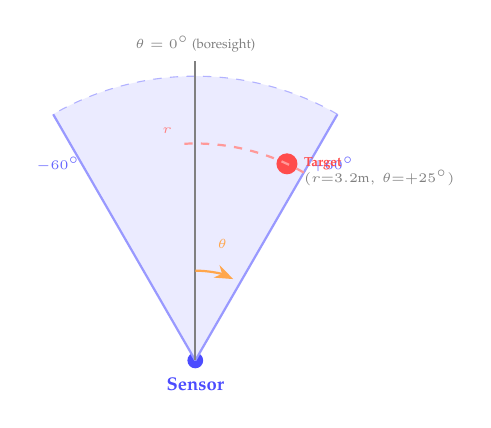
\begin{tikzpicture}[scale=0.95, transform shape]
				% Sensor origin
				\fill[blue!70] (0,0) circle (3pt);
				\node[below=3pt, font=\scriptsize\bfseries, text=blue!70] at (0,0) {Sensor};

				% FoV cone
				\fill[blue!8] (0,0) -- (60:3.8) arc (60:120:3.8) -- cycle;
				\draw[blue!40, thick] (0,0) -- (60:3.8);
				\draw[blue!40, thick] (0,0) -- (120:3.8);
				\draw[blue!30, dashed] (60:3.8) arc (60:120:3.8);

				% Boresight
				\draw[gray, thick] (0,0) -- (90:4.0);
				\node[above, font=\tiny, text=gray] at (90:4.0) {$\theta=0^{\circ}$ (boresight)};

				% Angle labels
				\node[font=\tiny, text=blue!60] at (55:3.2) {$+60^{\circ}$};
				\node[font=\tiny, text=blue!60] at (125:3.2) {$-60^{\circ}$};

				% Target point
				\fill[red!70] (65:2.9) circle (4pt);
				\node[right=3pt, font=\tiny\bfseries, text=red!70] at (65:2.9) {Target};
				\node[right=3pt, below right=-1pt and 3pt, font=\tiny, text=gray] at (65:2.9) {$(r{=}3.2\text{m},\ \theta{=}{+}25^{\circ})$};

				% Range arc
				\draw[red!40, dashed, thick] (60:2.9) arc (60:95:2.9);
				\node[font=\tiny, text=red!50] at (97:3.1) {$r$};

				% Angle arc
				\draw[-Stealth, orange!70, thick] (90:1.2) arc (90:65:1.2);
				\node[font=\tiny, text=orange!70] at (77:1.6) {$\theta$};
			\end{tikzpicture}
		\end{column}
	\end{columns}

	\begin{center}
		\small\textbf{Model output:} Predicted $(\hat{r}, \hat{\theta})$ in meters and degrees
	\end{center}
\end{frame}

%========================================================================================
%	SLIDE 7 ; FEATURE ENGINEERING
%========================================================================================

\section{ML Pipeline}

\begin{frame}
	\frametitle{Forward-Fill, Not Zero-Fill}
	\framesubtitle{Feature Engineering for Asynchronous Sensor Streams}

	\begin{columns}[c]
		\begin{column}{0.48\textwidth}
			\scriptsize
			\begin{alertblock}{Problem: Zero-Fill}
				Setting $r{=}0, \theta{=}0$ during radar dropout tells the network ``target is at the origin.'' The model \alert{pulls predictions toward $(0,0)$} during every dropout.
			\end{alertblock}

			\begin{exampleblock}{Forward-Fill Solution}
				\begin{itemize}
					\item Hold last valid reading during dropout
					\item Binary \texttt{fresh} flag tells model whether to trust the value
					\item Sliding window of 5 events $\to$ short-term consensus
				\end{itemize}
			\end{exampleblock}

			\medskip
			\textbf{5 features $\times$ 5 timesteps = 25 input values $\to$ MLP}
		\end{column}

		\begin{column}{0.48\textwidth}
			\centering
			\scriptsize
			\begin{tabular}{l c c c}
				\toprule
				\textbf{Event} & \textbf{radar\_r} & \textbf{fresh} & \textbf{wifi\_r} \\
				\midrule
				Radar valid & 2.08 & \alert{1.0} & 2.34\,\textsuperscript{fwd} \\
				Radar valid & 2.09 & \alert{1.0} & 2.34\,\textsuperscript{fwd} \\
				R.\ dropout & 2.09\,\textsuperscript{fwd} & \alert{0.0} & 2.34\,\textsuperscript{fwd} \\
				R.\ dropout & 2.09\,\textsuperscript{fwd} & \alert{0.0} & 2.34\,\textsuperscript{fwd} \\
				Wi-Fi arrives & 2.09\,\textsuperscript{fwd} & 0.0 & \alert{2.19} \\
				Radar returns & \alert{2.10} & \alert{1.0} & 2.19\,\textsuperscript{fwd} \\
				\bottomrule
			\end{tabular}
			\smallskip

			\tiny \textsuperscript{fwd} = held from last valid reading
		\end{column}
	\end{columns}
\end{frame}

%========================================================================================
%	SLIDE 8 ; ML MODEL ARCHITECTURE
%========================================================================================

\begin{frame}
	\frametitle{Float32 MLP ; Why Not INT8?}
	\framesubtitle{Compact Neural Architecture for Edge Deployment}

	\begin{columns}[c]
		\begin{column}{0.35\textwidth}
			\centering
			% TikZ MLP Architecture ; compact
			\begin{tikzpicture}[scale=0.8, transform shape,
				layer/.style={rectangle, rounded corners=3pt, draw=#1!70, fill=#1!12, minimum width=2.3cm, minimum height=0.65cm, font=\scriptsize\bfseries, align=center},
				layer/.default=blue]

				\node[layer=green!50!black] (input) at (0,0) {Input (25)};
				\node[layer=blue] (d1) at (0,-1.2) {Dense(48, ReLU)};
				\node[layer=blue] (d2) at (0,-2.4) {Dense(24, ReLU)};
				\node[layer=red!60!black] (out) at (0,-3.6) {Dense(2, Linear)};
				\node[font=\scriptsize, text=red!60!black] (outlbl) at (0,-4.4) {$[\hat{r}_{\text{norm}},\ \hat{\theta}_{\text{norm}}]$};

				\draw[dataflow] (input) -- (d1);
				\draw[dataflow] (d1) -- (d2);
				\draw[dataflow] (d2) -- (out);
				\draw[-Stealth, thick, draw=red!50] (out) -- (outlbl);
			\end{tikzpicture}
		\end{column}

		\begin{column}{0.60\textwidth}
			\scriptsize
			\begin{table}
				\centering
				\begin{tabular}{l l}
					\toprule
					\textbf{Property} & \textbf{Value} \\
					\midrule
					Parameters & 2,474 \\
					Model size & 11.6\,KB (.tflite) \\
					Precision & \alert{Float32} (no quant.) \\
					Output act. & Linear \\
					Inference time & $\sim$350\,$\mu$s on ESP32-S3 \\
					\bottomrule
				\end{tabular}
			\end{table}

			\smallskip
			\begin{alertblock}{Why Float32, not INT8?}
				\begin{itemize}
					\item INT8: 256 bins over 6\,m = 2.35\,cm floor
					\item Error \alert{compounds} through every hidden layer
					\item tanh LUT deviates 30\%+ from true values
					\item At 11.6\,KB, quantization saves \textbf{nothing} but destroys regression accuracy
				\end{itemize}
			\end{alertblock}
		\end{column}
	\end{columns}
\end{frame}

%========================================================================================
%	SLIDE 9 ; TRAINING PIPELINE
%========================================================================================

\begin{frame}
	\frametitle{Data $\to$ Features $\to$ Model $\to$ Deployment}
	\framesubtitle{End-to-End Training Pipeline}

	\centering
	% TikZ Training Pipeline ; compact layout to avoid overlap
	\begin{tikzpicture}[scale=0.75, transform shape]
		\node[pipeblock=green!50!black] (data) at (0,0) {Manual Data\\Collection};
		\node[pipeblock=blue] (feat) at (2.8,0) {Feature\\Engineering};
		\node[pipeblock=purple] (train) at (5.6,0) {Training\\(Keras)};
		\node[pipeblock=orange] (conv) at (8.4,0) {Conversion\\(TFLite)};
		\node[pipeblock=red!60!black] (deploy) at (8.4,-2.5) {ESP32-S3\\TFLite Micro};

		\draw[dataflow] (data) -- (feat);
		\draw[dataflow] (feat) -- (train);
		\draw[dataflow] (train) -- (conv);
		\draw[dataflow] (conv) -- (deploy);

		% Annotations below ; reduced text width, clear of deploy box
		\node[annot, below=0.12cm of data, text width=1.8cm, align=center] {12 static poses\\30s each\\Micro-motion\\Polar ground truth};
		\node[annot, below=0.12cm of feat, text width=1.8cm, align=center] {Forward-fill\\Normalize [0,1]\\Window = 5\\Split by segment};
		\node[annot, below=0.12cm of train, text width=1.8cm, align=center] {EarlyStopping\\ReduceLR\\MSE loss\\200 epochs max};
		\node[annot, below=0.12cm of conv, text width=1.8cm, align=center] {Pure Float32\\No quantization\\xxd $\to$ C header\\alignas(16)};
	\end{tikzpicture}

	\medskip

	\begin{columns}[c]
		\begin{column}{0.45\textwidth}
			\begin{block}{Dataset}
				$\sim$35,000 events across 12 segments (8 clear + 4 occluded)
			\end{block}
		\end{column}
		\begin{column}{0.45\textwidth}
			\begin{block}{Split}
				70\% train / 15\% val / 15\% test ; split by \alert{segment}, not by row
			\end{block}
		\end{column}
	\end{columns}
\end{frame}

%========================================================================================
%	NEW SLIDE ; PHYSICAL SETUP
%========================================================================================

\begin{frame}
	\frametitle{Physical Setup \& Data Acquisition}
	\framesubtitle{Markers and Positioning for Ground Truth Collection}

	\begin{columns}[c]
		\begin{column}{0.45\textwidth}
			\scriptsize
			\textbf{Data Collection Protocol:}
			\begin{itemize}
				\item \textbf{Ground Truth Markers:} 12 precisely measured points across the room
				\item \textbf{Target Positioning:} ESP32-S3 tag + corner reflector moved through grid
				\item \textbf{Environment:} Typical hostel room with dense obstacles (furniture/objects)
				\item \textbf{Capturing Variance:} 30s capture per pose to record micro-motion Doppler shifts
			\end{itemize}

			\medskip
			\begin{exampleblock}{Goal}
				Generate a high-fidelity dataset of $(r, \theta, \text{fresh})$ features with polar ground truth $(\hat{r}, \hat{\theta})$.
			\end{exampleblock}
		\end{column}

		\begin{column}{0.52\textwidth}
			\centering
			\begin{figure}
				\includegraphics[width=\linewidth, height=0.7\textheight, keepaspectratio]{data_acquistion_training for_ml.png}
				\caption{Indoor lab environment with ground truth markers}
			\end{figure}
		\end{column}
	\end{columns}
\end{frame}

%========================================================================================
%	SLIDE 10 ; RESULTS: MODEL ACCURACY
%========================================================================================

\section{Results \& Analysis}

\begin{frame}
	\frametitle{Fusion Accuracy ; Test Set}
	\framesubtitle{Model Performance Metrics}

	\begin{columns}[c]
		\begin{column}{0.50\textwidth}
			\scriptsize
			\begin{table}
				\centering
				\begin{tabular}{l c c c}
					\toprule
					\textbf{Metric} & \textbf{Train} & \textbf{Val} & \textbf{Test} \\
					\midrule
					MSE (norm) & 0.000588 & 0.000621 & 0.001958 \\
					MAE range (m) & 0.107 & 0.078 & \alert{\textbf{0.118}} \\
					MAE angle ($^{\circ}$) & 2.09 & 3.02 & \alert{\textbf{4.88}} \\
					Euclid.\ mean (m) & 0.168 & 0.144 & \alert{\textbf{0.256}} \\
					Euclid.\ 95th\% (m) & 0.385 & 0.276 & \alert{\textbf{0.555}} \\
					\bottomrule
				\end{tabular}
				\caption{Model accuracy metrics}
			\end{table}
		\end{column}

		\begin{column}{0.45\textwidth}
			\begin{figure}
				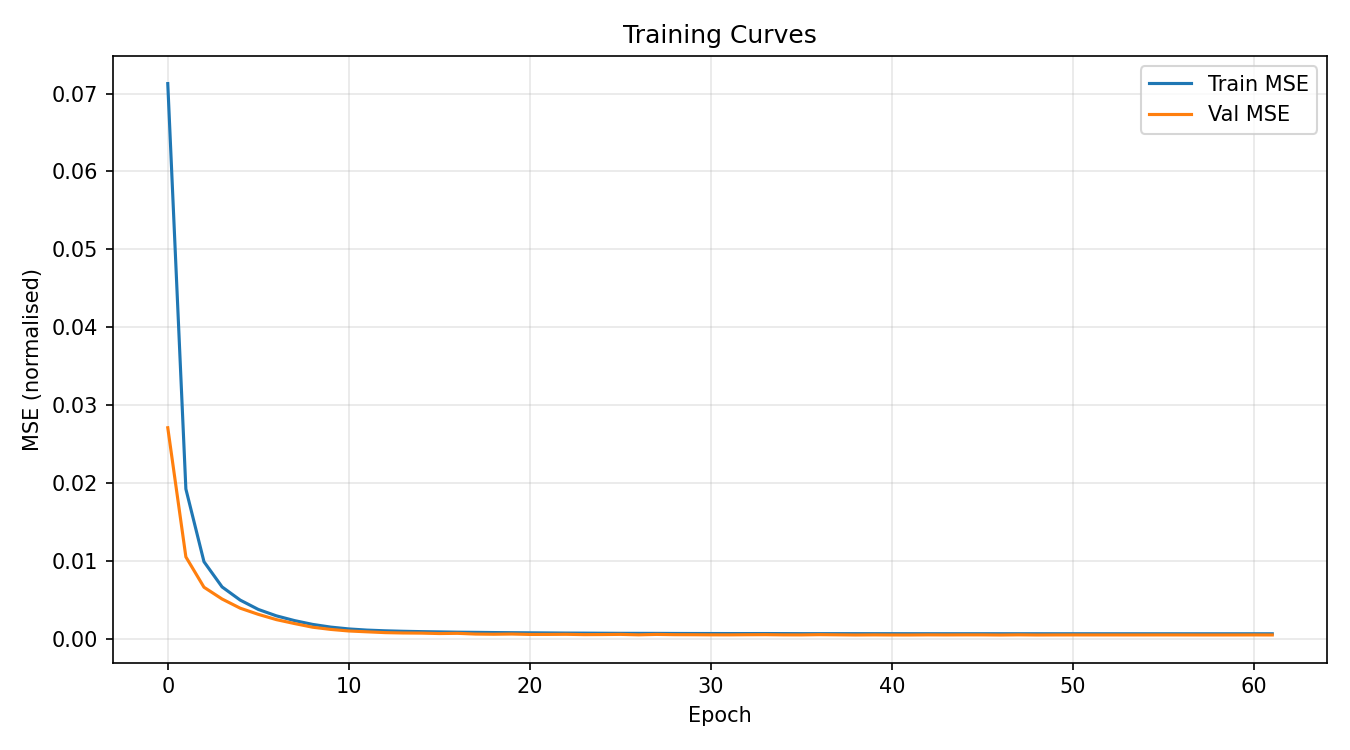
\includegraphics[width=\linewidth, height=0.50\textheight, keepaspectratio]{training_cuve.png}
				\caption{Training loss curve}
			\end{figure}
		\end{column}
	\end{columns}
\end{frame}

%========================================================================================
%	SLIDE 11 ; RESULTS: ERROR BY DISTANCE
%========================================================================================

\begin{frame}
	\frametitle{Accuracy Across Distance Bands}
	\framesubtitle{Near-Field vs Far-Field Performance}

	\begin{columns}[c]
		\begin{column}{0.40\textwidth}
			\scriptsize
			\begin{table}
				\centering
				\begin{tabular}{l c c c}
					\toprule
					\textbf{Band} & \textbf{N} & \textbf{MAE r} & \textbf{MAE $\theta$} \\
					\midrule
					2--3\,m & 566 & 0.116 & 6.66$^{\circ}$ \\
					3--5\,m & 794 & 0.119 & 3.62$^{\circ}$ \\
					\bottomrule
				\end{tabular}
				\caption{Error by distance band}
			\end{table}
		\end{column}

		\begin{column}{0.55\textwidth}
			\begin{figure}
				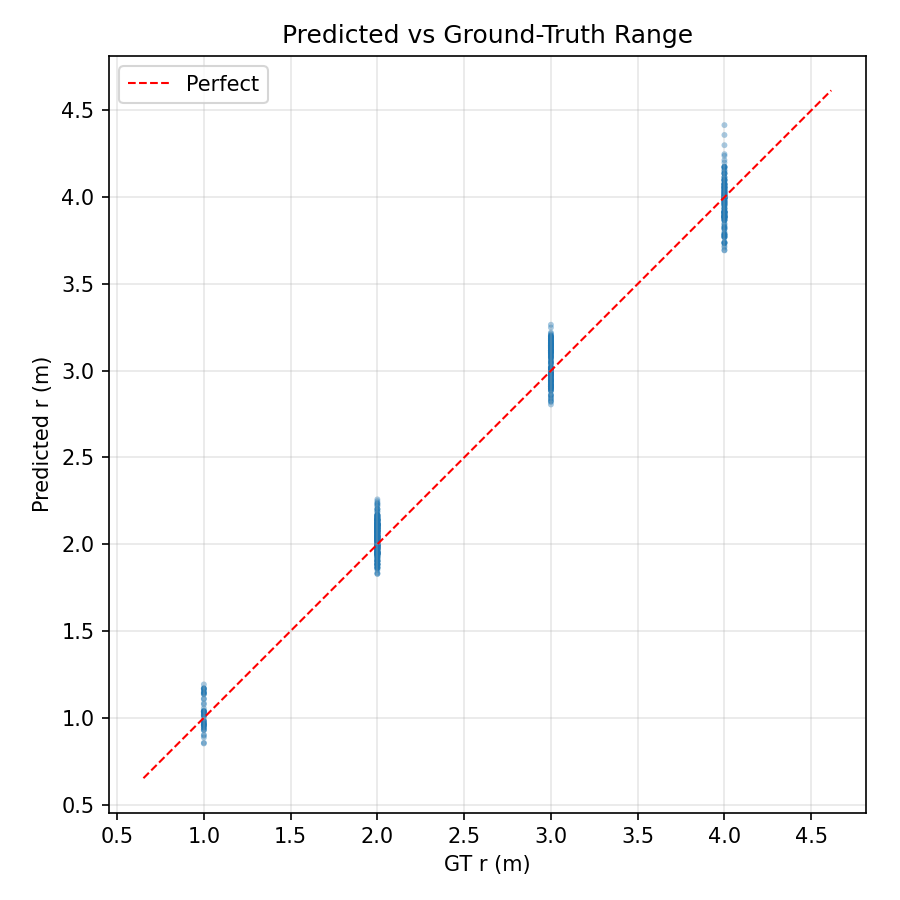
\includegraphics[width=0.46\linewidth, height=0.42\textheight, keepaspectratio]{predVgndTruth_r.png}
				\hfill
				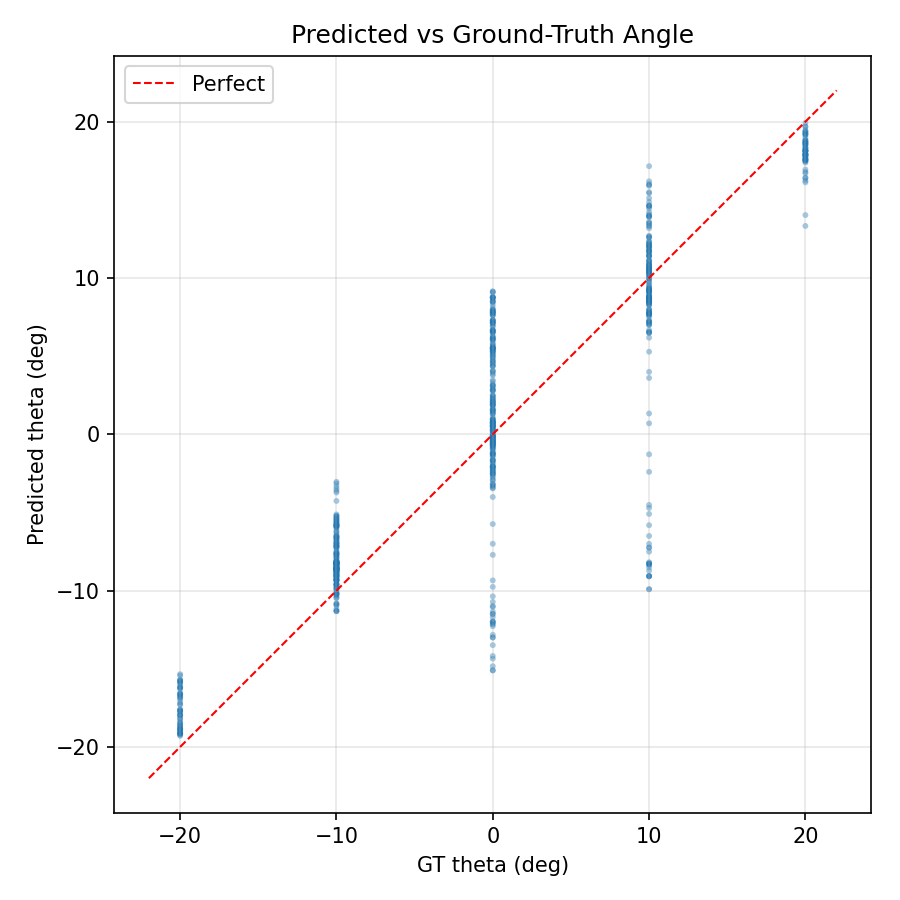
\includegraphics[width=0.46\linewidth, height=0.42\textheight, keepaspectratio]{predVgndTruth_theta.png}
				\caption{Predicted vs ground truth ($r$ left, $\theta$ right)}
			\end{figure}
		\end{column}
	\end{columns}
\end{frame}

%========================================================================================
%	SLIDE 12 ; RESULTS: SENSOR COMPARISON
%========================================================================================

\begin{frame}
	\frametitle{Fused Output vs Raw Sensors}
	\framesubtitle{ML Fusion Inherits Best of Both Worlds}

	\begin{columns}[c]
		\begin{column}{0.50\textwidth}
			\scriptsize
			\begin{table}
				\centering
				\begin{tabular}{l c c c}
					\toprule
					\textbf{Source} & \textbf{MAE r (m)} & \textbf{Angle?} & \textbf{Walls?} \\
					\midrule
					Raw Radar & $\pm$0.15--0.65 & Yes & No \\
					Raw Wi-Fi FTM & $\pm$1.1--4.8 & No & Yes \\
					\textbf{ML Fusion} & \alert{\textbf{0.118}} & \alert{Yes} & \alert{Yes} \\
					\bottomrule
				\end{tabular}
				\caption{Sensor comparison}
			\end{table}

			\smallskip
			\begin{exampleblock}{Key Result}
				Fusion maintains \textbf{sub-20\,cm} range accuracy while inheriting Wi-Fi's wall-penetration capability.
			\end{exampleblock}
		\end{column}

		\begin{column}{0.45\textwidth}
			\scriptsize
			\begin{table}
				\centering
				\begin{tabular}{l c c}
					\toprule
					\textbf{Condition} & \textbf{N} & \textbf{Euclid.\ MAE} \\
					\midrule
					Radar available & 1,163 & 0.262\,m \\
					Radar occluded & 197 & 0.226\,m \\
					\bottomrule
				\end{tabular}
				\caption{Performance during occlusion}
			\end{table}

			\smallskip
			\begin{block}{Adaptive Trust}
				Model seamlessly shifts trust to Wi-Fi when radar drops out ; \alert{no manual switching} logic.
			\end{block}
		\end{column}
	\end{columns}
\end{frame}

%========================================================================================
%	SLIDE 13 ; RESULTS: EDGE DEPLOYMENT
%========================================================================================

\begin{frame}
	\frametitle{Inference Performance on ESP32-S3}
	\framesubtitle{Edge Deployment Metrics}

	\begin{columns}[c]
		\begin{column}{0.45\textwidth}
			\scriptsize
			\begin{table}
				\centering
				\begin{tabular}{l l}
					\toprule
					\textbf{Metric} & \textbf{Value} \\
					\midrule
					Model file size & 11.6\,KB \\
					Tensor arena & 32\,KB (internal SRAM) \\
					Inference latency & $\sim$350\,$\mu$s \\
					Real-time budget & 50,000\,$\mu$s (50\,ms) \\
					Headroom & \alert{\textbf{99.3\%} unused} \\
					Conversion loss & $1.79 \times 10^{-7}$ \\
					Framework & TFLite Micro, Float32 \\
					\bottomrule
				\end{tabular}
				\caption{ESP32-S3 inference benchmarks}
			\end{table}
		\end{column}

		\begin{column}{0.50\textwidth}
			\begin{figure}
				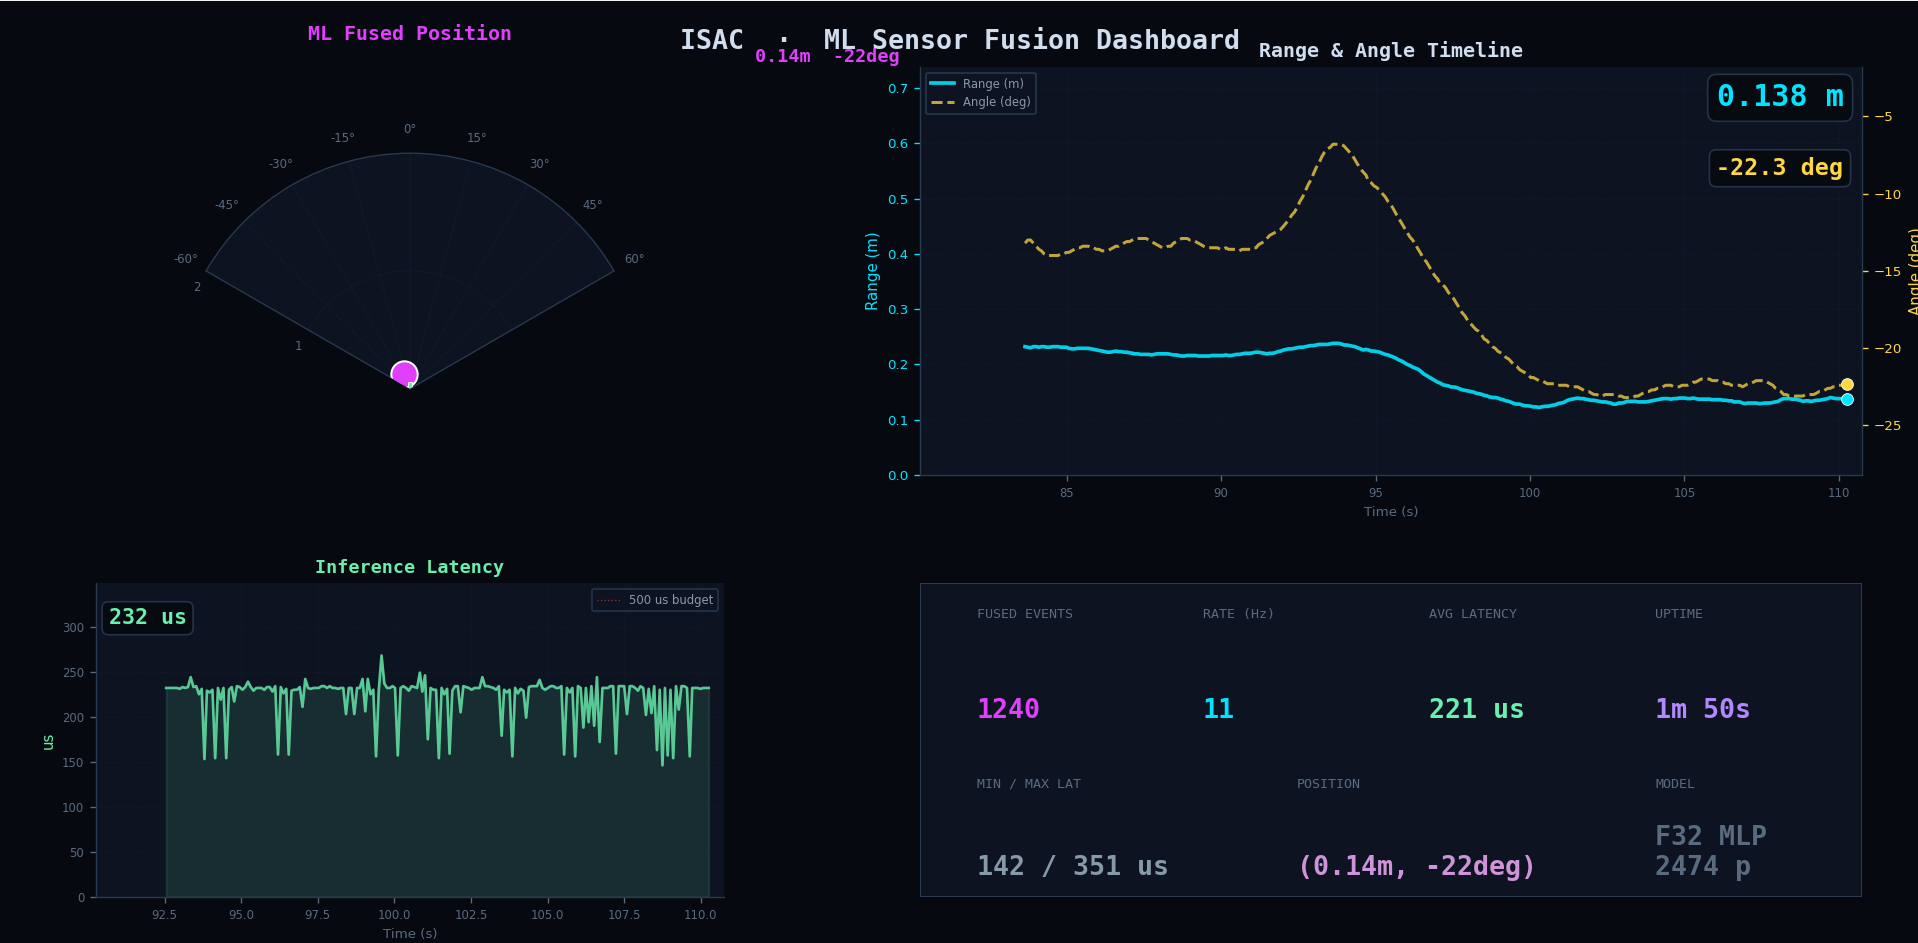
\includegraphics[width=\linewidth, height=0.50\textheight, keepaspectratio]{Dashboard-fusedWithInferenceTimes.png}
				\caption{ESP32-S3 serial output showing FUSED predictions}
			\end{figure}
		\end{column}
	\end{columns}
\end{frame}

%========================================================================================
%	SLIDE 14 ; RESULTS: MULTIPATH MITIGATION
%========================================================================================

\begin{frame}
	\frametitle{HT40 + Min-RTT Filtering}
	\framesubtitle{Multipath Mitigation Strategy}

	\begin{columns}[c]
		\begin{column}{0.50\textwidth}
			\scriptsize
			\begin{enumerate}
				\item Force \textbf{40\,MHz} (HT40) bandwidth $\to$ resolution floor drops to \alert{3.75\,m}
				\item 16 frames per FTM burst $\to$ collect 16 RTT measurements
				\item Take the \textbf{minimum RTT} $\to$ closest to true line-of-sight path
			\end{enumerate}

			\medskip
			\begin{alertblock}{Without HT40}
				2.4\,GHz Wi-Fi at 20\,MHz $\to$ theoretical resolution floor of 7.5\,m. Indoor multipath adds 1--3\,m bias.
			\end{alertblock}
		\end{column}

		\begin{column}{0.46\textwidth}
			\centering
			% TikZ Min-RTT visualization ; scaled down, labels inside chart area
			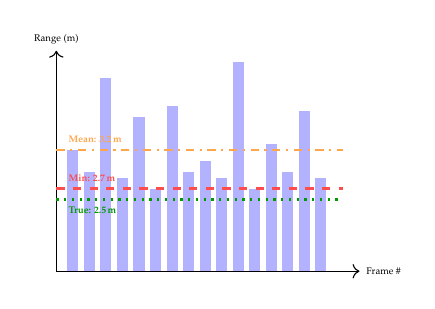
\begin{tikzpicture}[scale=0.7, transform shape]
				% Bar chart showing raw vs filtered
				\draw[->] (0,0) -- (0,4) node[above, font=\tiny] {Range (m)};
				\draw[->] (0,0) -- (5.5,0) node[right, font=\tiny] {Frame \#};

				% Raw samples (16 bars)
				\foreach \x/\h in {0.3/2.2, 0.6/1.8, 0.9/3.5, 1.2/1.7, 1.5/2.8, 1.8/1.5, 2.1/3.0, 2.4/1.8, 2.7/2.0, 3.0/1.7, 3.3/3.8, 3.6/1.5, 3.9/2.3, 4.2/1.8, 4.5/2.9, 4.8/1.7} {
					\fill[blue!30] (\x-0.1, 0) rectangle (\x+0.1, \h);
				}

				% Min line ; label inside chart area
				\draw[red!70, thick, dashed] (0, 1.5) -- (5.2, 1.5);
				\node[font=\tiny\bfseries, text=red!70, anchor=south west] at (0.1, 1.5) {Min: 2.7\,m};

				% True distance line
				\draw[green!60!black, thick, dotted] (0, 1.3) -- (5.2, 1.3);
				\node[font=\tiny\bfseries, text=green!60!black, anchor=north west] at (0.1, 1.3) {True: 2.5\,m};

				% Mean line
				\draw[orange!70, thick, dashdotted] (0, 2.2) -- (5.2, 2.2);
				\node[font=\tiny\bfseries, text=orange!70, anchor=south west] at (0.1, 2.2) {Mean: 3.2\,m};
			\end{tikzpicture}
		\end{column}
	\end{columns}
\end{frame}

%========================================================================================
%	SLIDE 15 ; CHALLENGES & SOLUTIONS
%========================================================================================

\section{Challenges \& Solutions}

\begin{frame}
	\frametitle{Key Technical Challenges}
	\framesubtitle{Problems Encountered \& How They Were Solved}

	\centering
	\scriptsize
	\begin{tabular}{c p{2.1cm} p{2.9cm} p{3.6cm}}
		\toprule
		\textbf{\#} & \textbf{Challenge} & \textbf{Root Cause} & \textbf{Solution} \\
		\midrule
		1 & Radar drops stationary targets & LD2450 MTI filter needs Doppler shift & Micro-motion protocol ; subjects sway gently \\[3pt]
		2 & UART corruption during FTM & Wi-Fi ISR preempts UART on same core, FIFO overflows & UART on Core 1, Wi-Fi on Core 0 \\[3pt]
		3 & INT8 quant.\ destroys accuracy & 256 bins / 6\,m = 2.35\,cm floor; tanh LUT 30\%+ off & Stay \alert{Float32} ; 11.6\,KB \\[3pt]
		4 & Zero-fill pulls to origin & $r{=}0$ means ``at sensor'' not ``unknown'' & \alert{Forward-fill} + binary fresh flag \\[3pt]
		5 & Wi-Fi multipath inflates range & 2.4\,GHz reflects, 20\,MHz can't resolve & \alert{HT40} + min-RTT filter \\
		\bottomrule
	\end{tabular}
\end{frame}

%========================================================================================
%	SLIDE 16 ; REMAINING WORK
%========================================================================================

\section{Remaining Work}

\begin{frame}
	\frametitle{Remaining $\sim$15\%}
	\framesubtitle{From Current State to Final Validation}

	\scriptsize
	\begin{table}
		\centering
		\begin{tabular}{l l p{5.5cm}}
			\toprule
			\textbf{Task} & \textbf{Status} & \textbf{Details} \\
			\midrule
			Extended range data & Pending & Current: 2--5\,m only. Need 0.5--2\,m and 5--6\,m segments \\[3pt]
			Hardware packaging & Pending & 3D-print PLA enclosures, vertical stacking to reduce EM coupling \\[3pt]
			Multi-tag testing & Pending & 2--3 simultaneous tags ; ESP-NOW collision handling \\[3pt]
			Field validation & Pending & Walk-tests in warehouse / factory environment \\
			\bottomrule
		\end{tabular}
	\end{table}

	\medskip

	\begin{alertblock}{Known Limitation}
		\scriptsize Wi-Fi FTM provides \alert{no angle}. During full radar blackout, range accuracy is maintained but angular estimate relies on stale forward-fill. A second angle-capable sensor (UWB, camera) would resolve this.
	\end{alertblock}
\end{frame}

%========================================================================================
%	SLIDE 17 ; REFERENCES
%========================================================================================

\section{References}

\begin{frame}
	\frametitle{Key References}

	\scriptsize
	\begin{columns}[t]
		\begin{column}{0.48\textwidth}
			\begin{enumerate}
				\item \textbf{Pegoraro et al.\ (2023)} ; SPARROW: mmWave radar occlusion characterization
				\item \textbf{Wang et al.\ (2022)} ; ISAC for 6G: principles and applications
				\item \textbf{Chen, Arambel \& Mehra (2002)} ; Covariance Intersection for distributed fusion
				\item \textbf{Aggarwal et al.\ (2022)} ; IEEE 802.11mc FTM ranging evaluation
				\item \textbf{Zubow et al.\ (2023)} ; FTM-based indoor localization
			\end{enumerate}
		\end{column}
		\begin{column}{0.48\textwidth}
			\begin{enumerate}
				\setcounter{enumi}{5}
				\item \textbf{Hoang et al.\ (2025)} ; Wi-Fi FTM survey
				\item \textbf{Gaiba et al.\ (2024)} ; ESP32 Wi-Fi sensing platform
				\item \textbf{Espressif (2024)} ; ESP-IDF v5.2 FTM programming guide
				\item \textbf{David et al.\ (2022)} ; TFLite Micro deployment on embedded MCUs
				\item \textbf{HiLink (2024)} ; HLK-LD2450 datasheet \& UART protocol
			\end{enumerate}
		\end{column}
	\end{columns}
\end{frame}

%========================================================================================
%	CLOSING SLIDE
%========================================================================================

\begin{frame}[plain]
	\begin{center}
		{\Huge Thank You!}

		\bigskip\bigskip

		{\LARGE Questions? Comments?}

		\vfill
		\small \textit{ML-Based Asynchronous Sensor Fusion for Indoor Localization} \\
		\small Edge-Deployed Neural Fusion on ESP32-S3 ISAC Nodes
	\end{center}
\end{frame}

%----------------------------------------------------------------------------------------

\end{document}
